\chapter{The background cosmology}\label{ch:background}
\chapterstatus{written}{2026-11-17}

The expansion history of a homogeneous and isotropic universe is the input of almost everything else in the library:
the recombination rates compete with the expansion rate, the perturbation equations contain $\Hp$ and its derivatives,
the line-of-sight integrals need the distance to the last-scattering surface, simulations need $H(a)$ for their time
steps and growth factors, and survey and lensing calculations need distances. \fml{} has one implementation of the
background, \cls{Background} in \file{Cosmology/Background}, which all these users share. This chapter describes its
equations, the species and theories of gravity it is built from, the model library and the numerical methods.

\begin{modulebox}{Cosmology/Background}
Namespace \nsp{FML::COSMOLOGY::BACKGROUND}; header-only (needs \file{Spline}, \file{ODESolver}, \file{Math}, GSL).\par
Core: \file{Background.h} (abstract interface, times and distances), \file{ComponentBackground.h} (species + field
equations), \file{TabulatedBackground.h}, \file{FunctionBackground.h}, \file{BackgroundParameters.h}.\par
Species and gravity: \file{Species.h}, \file{FieldEquations.h}, \file{FieldEquation_GeneralRelativity.h},
\file{FieldEquation_DGP.h}, \file{FieldEquation_BransDicke.h}.\par
Models: \file{BackgroundModel_<name>.h} for LCDM, w0wa, DGP, Quintessence, EDE, Axion, BransDicke,
CoupledQuintessence, CubicGalileon, DarkScattering, IDE, Tabulated, HorndeskiTable; the registry \file{Presets.h}.\par
Solver interface: \file{BackgroundCosmology.h/.cpp} (SI adapter used by the Einstein--Boltzmann solver),
\file{CosmologyParameters.h/.cpp}, \file{BBN.h/.cpp}.\par
Documentation: \file{Cosmology/Background/README.md}. Tests: \file{Cosmology/Background/tests}.
\end{modulebox}

\section{The Friedmann equations}\label{sec:bg-friedmann}

On large scales the universe is described by the Friedmann--Lema\^itre--Robertson--Walker metric,
\begin{equation}
\dd s^2=-c^2\dd t^2+a^2(t)\left[\frac{\dd r^2}{1-Kr^2}+r^2\dd\Omega^2\right],
\end{equation}
with the scale factor $a(t)$, normalised to $a_0=1$ today, and the spatial curvature $K$ ($K>0$ closed, $K<0$ open).
Homogeneity and isotropy restrict the matter to perfect fluids with energy densities $\rho_ic^2$ and pressures $p_i$.
In general relativity Einstein's equations reduce to the Friedmann equation and the acceleration equation,
\begin{equation}
H^2\equiv\left(\frac{\dot a}{a}\right)^2=\frac{8\pi G}{3}\sum_i\rho_i-\frac{Kc^2}{a^2},\qquad
\frac{\ddot a}{a}=-\frac{4\pi G}{3}\sum_i\left(\rho_i+\frac{3p_i}{c^2}\right).
\label{eq:bg-friedmann}
\end{equation}
Their combination is the continuity equation. With the time variable $x=\ln a$ used throughout the library and
$'=\dd/\dd x$,
\begin{equation}
\rho_i'=-3\left(\rho_i+\frac{p_i}{c^2}\right)\qquad\text{(uncoupled species)},
\label{eq:bg-continuity}
\end{equation}
which for a constant equation of state $w_i=p_i/(\rho_ic^2)$ gives $\rho_i\propto a^{-3(1+w_i)}$. Species that
exchange energy (interacting dark energy, coupled quintessence) replace \cref{eq:bg-continuity} by their own
equations, but the sum over all species still obeys it.

Measuring densities in units of today's critical density $\rho_{c0}=3H_0^2/(8\pi G)$ and writing $E=H/H_0$, the
Friedmann equation of GR becomes
\begin{equation}
E^2(x)=\sum_i\frac{\rho_i(x)}{\rho_{c0}}+\Om_ke^{-2x},\qquad \Om_k=-\frac{Kc^2}{H_0^2},
\label{eq:bg-E2}
\end{equation}
and $E(0)=1$ is the closure condition $\sum_i\Om_i+\Om_k=1$. For the standard species this is the familiar
\begin{equation}
E^2=\Om_\gamma e^{-4x}+\Om_\nu e^{-4x}+(\Om_b+\Om_{\rm cdm})e^{-3x}+\frac{\rho_{\nu,\rm massive}}{\rho_{c0}}
+\Om_ke^{-2x}+\Om_\Lambda .
\end{equation}
The density parameters at time $x$ are $\Om_i(x)=\rho_i(x)/(\rho_{c0}E^2)$, and curvature is reported as
$\Om_k(x)=\Om_ke^{-2x}/E^2$, so that $\sum_i\Om_i(x)+\Om_k(x)=1$ in GR (in Brans--Dicke gravity the scalar field
has no species and the sum differs from one, \cref{sec:bg-bransdicke}). From $E$ and its logarithmic derivative the
library derives
\begin{equation}
\Hp\equiv aH,\qquad w_{\rm eff}=-1-\frac23\frac{\dd\ln E}{\dd x},\qquad q=-\frac{\ddot aa}{\dot a^2}=-1-\frac{\dd\ln E}{\dd x},
\end{equation}
the effective equation of state of the total (curvature counted as a fluid with $w=-1/3$) and the deceleration
parameter. The onset of acceleration is where $\Hp'=0$.

\paragraph*{Radiation.} The photons are a blackbody of temperature $T_{\rm CMB}$ (default $2.7255$\,K), so
\begin{equation}
\Om_\gamma=\frac{\pi^2}{15}\frac{(k_BT_{\rm CMB})^4}{(\hbar c)^3}\frac{1}{\rho_{c0}c^2}.
\end{equation}
Neutrinos decoupled before electron--positron annihilation, after which $T_\nu=(4/11)^{1/3}T_\gamma$; with the
fermionic factor $7/8$ each massless species contributes $\frac78(4/11)^{4/3}\Om_\gamma$. The effective number
$N_{\rm eff}$ (default $3.046$; $3.044$ is the modern value) counts \emph{all} neutrinos. A massive species of
temperature $T_{\rm ncdm}=0.71611\,T_{\rm CMB}$ (CLASS's default) contributes
\begin{equation}
N_{\rm ncdm}=\left(\frac{T_{\rm ncdm}/T_{\rm CMB}}{(4/11)^{1/3}}\right)^4=1.0132
\end{equation}
to $N_{\rm eff}$, and the remaining $N_{\rm eff}-n_{\rm massive}N_{\rm ncdm}$ species are massless. This is the
convention of CLASS and of the Einstein--Boltzmann solver (\cref{ch:linear-perturbations}); with it a massive species
has $\Om_\nu h^2=m_\nu/93.14\,$eV today.

\section{Times, horizons and distances}\label{sec:bg-distances}

\paragraph*{Clocks.} Cosmic time $t$, conformal time $\eta$ and the comoving distance $\chi$ to an object at $x$
obey
\begin{equation}
\frac{\dd t}{\dd x}=\frac{1}{H},\qquad \frac{\dd\eta}{\dd x}=\frac{c}{\Hp}=\frac{c}{aH},\qquad \chi(x)=\eta_0-\eta(x).
\label{eq:bg-clocks}
\end{equation}
$\eta(x)$ is the particle horizon, the comoving distance light has travelled since the big bang; $c/\Hp$ is the
comoving Hubble radius, and a mode of wavenumber $k$ is outside the horizon while $ck<\Hp$. In an era dominated by a
single component with $\rho\propto a^{-n}$,
\begin{equation}
\frac{\Hp'}{\Hp}=1-\frac n2,\qquad \frac{\Hp''}{\Hp}=\left(1-\frac n2\right)^2,\qquad
\frac{\eta\Hp}{c}=\frac{2}{n-2}\;(n>2),\qquad t=\frac{2}{nH},
\label{eq:bg-single}
\end{equation}
i.e.\ $\eta\Hp/c=1$ in radiation domination and $2$ in matter domination. These limits are both the initial
conditions of the integration and the main tests of it.

\paragraph*{Distances.} In a curved universe the comoving transverse distance of an object at comoving radial
distance $\chi$ is
\begin{equation}
D_M=\sin_K(\chi)=\begin{cases}\sin(\sqrt K\chi)/\sqrt K & K>0\ \text{(closed)}\\ \chi & K=0\\
\sinh(\sqrt{-K}\chi)/\sqrt{-K} & K<0\ \text{(open)}\end{cases},\qquad
\cot_K(\chi)=\frac{\dd\ln\sin_K\chi}{\dd\chi},
\label{eq:bg-sinK}
\end{equation}
and the angular diameter, luminosity and Hubble distances are
\begin{equation}
D_A=\frac{D_M}{1+z},\qquad D_L=(1+z)D_M,\qquad D_H=\frac{c}{H}.
\end{equation}
$\sin_K$ and $\cot_K$ are evaluated with series expansions when $|K\chi^2|<10^{-4}$, so that every quantity is
smooth through $\Om_k=0$; the same functions enter the line-of-sight integrals and the truncation of the Boltzmann
hierarchies in curved universes (\cref{ch:linear-perturbations,ch:cmb-spectra}).

\begin{implementation}[Implementation: tabulating times and distances]
A derived class provides the \emph{virtual core} --- $E(x)$, $\dd\ln E/\dd x$, $\Om_i(x)$, the parameters and the
valid range $[x_{\min},x_{\max}]$ (default $a\in[10^{-10},10]$) --- and calls \code{finalize()} at the end of its
constructor. \code{finalize()} integrates \cref{eq:bg-clocks} once:
\begin{itemize}
\item on a grid in $x$ with a node at $x=0$ and \code{points_per_unit_x} (default 200) points per unit $x$, with
      5-point Gauss--Legendre quadrature on each interval;
\item starting from the exact power-law solution at $x_{\min}$, which must lie in an era with $E\propto a^{-n/2}$,
      $n>2$: $\eta(x_{\min})=c/[aH_0E(n/2-1)]$ and $t(x_{\min})=2/(nH)$ (\cref{eq:bg-single});
\item computing $\chi=\eta_0-\eta$ by summation from $x=0$, which avoids the cancellation of two large numbers at
      low redshift.
\end{itemize}
$\ln\eta$, $\ln t$ and $\chi$ are stored as cubic splines, and the inverse $x(\chi)$ is splined on the reversed
arrays. In the far future of models whose $E$ grows very fast (e.g.\ CPL with $w_a>0$) $\chi$ stops changing in
double precision, and the inverse covers only the part where $\chi$ is strictly monotonic. Everything else
(distances with curvature, $a$- and $z$-versions of all functions, \code{info()}, \code{output()}) is non-virtual and
shared by all backgrounds. A \cls{Background} is immutable after construction and shared as
\code{std::shared_ptr<const Background>}; all methods are \code{const} and thread-safe.
\end{implementation}

\paragraph*{Units.} $E$ is dimensionless. The conformal time $\eta$, the comoving distance $\chi$ and all other distances
are in $\Mpch$, with $c/H_0=2997.92458\,\Mpch$. Cosmic time is in Gyr (\code{t_Gyr}, \code{age_Gyr}) or in units of $1/H_0$
(\code{t_H0}); the curvature
\code{K_hmpc2()} is in $(h/\mathrm{Mpc})^2$. Every function exists in versions taking $x$, $a$ or $z$.

\begin{figure}[htbp]
\centering
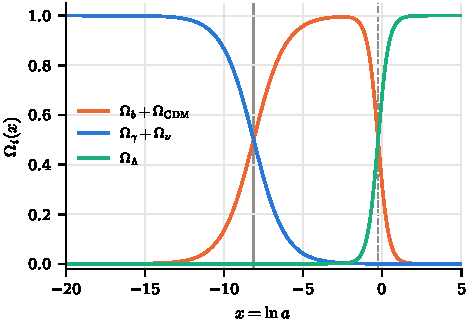
\includegraphics[width=0.49\textwidth]{m1_Omegas}\hfill
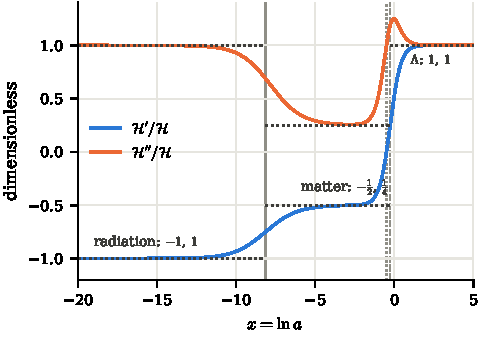
\includegraphics[width=0.49\textwidth]{m1_Hp_derivatives}
\caption{\emph{Left:} density parameters of radiation, matter and the cosmological constant in the fiducial
$\Lambda$CDM model ($h=0.67$, $\Om_b=0.05$, $\Om_{\rm cdm}=0.267$). \emph{Right:} $\Hp'/\Hp$ and $\Hp''/\Hp$ with
the analytic values of \cref{eq:bg-single} in each era (dotted). Vertical lines mark radiation--matter equality,
matter--$\Lambda$ equality and the onset of acceleration. From the Einstein--Boltzmann solver report.}
\label{fig:bg-omegas}
\end{figure}

\section{Species}\label{sec:bg-species}

A \cls{ComponentBackground} is a list of species (\file{Species.h}) and a theory of gravity
(\cref{sec:bg-field-equations}). A species gives its energy density $\rho(x)$ and pressure $p(x)$ in units of
$\rho_{c0}$ (pressure in $\rho_{c0}c^2$), its derivative $\rho'(x)$ (default: \cref{eq:bg-continuity}) and its second
derivative $\rho''$ (used by the perturbations of some theories; analytic for all species in the library, otherwise a
5-point central difference of $\rho'$ with step $10^{-3}$). Each species belongs to a component (\code{Baryons},
\code{CDM}, \code{Photons}, \code{MasslessNeutrinos}, \code{MassiveNeutrinos}, \code{DarkEnergy}, \code{Axions},
\code{Other}, \ldots), and $\Om(c,x)$ sums the species of component $c$. Matter, \code{Omega_m}, is baryons + CDM +
massive neutrinos (including their small relativistic part); an ultralight axion is a separate component, included
in \code{Omega_m_axion}. The function \code{standard_species(p)} gives the species every model has: baryons, CDM,
photons, massless neutrinos and one species per entry of \code{m_nu_eV}.

\subsection{Power laws and CPL dark energy}

\cls{PowerLawSpecies} has $\rho=\Om_0a^{-n}$ and $p=(n/3-1)\rho$: baryons and CDM ($n=3$), photons and massless
neutrinos ($n=4$) and a cosmological constant ($n=0$). \cls{CPLDarkEnergy} has the equation of state of Chevallier,
Polarski and Linder \cite{ChevallierPolarski2001,Linder2003}, $w(a)=w_0+w_a(1-a)$, for which \cref{eq:bg-continuity}
integrates to
\begin{equation}
\rho_{\rm DE}=\Om_{\rm DE}\,a^{-3(1+w_0+w_a)}e^{-3w_a(1-a)},\qquad
\rho_{\rm DE}''=3w_aa\,\rho_{\rm DE}+9(1+w)^2\rho_{\rm DE}.
\end{equation}

\subsection{Massive neutrinos}\label{sec:bg-ncdm}

Massive neutrinos decoupled while relativistic and keep the relativistic Fermi--Dirac distribution
$f_0(q)=1/(e^q+1)$ in the comoving momentum $q=ap/(k_BT_{\nu0})$ also after they become non-relativistic
\cite{LesgourguesPastor2006}. With the mass in units of the temperature, $M(x)=m_\nu c^2a/(k_BT_{\nu0})$, and the
comoving energy $\epsilon=\sqrt{q^2+M^2}$, one species (neutrino and antineutrino) has
\begin{gather}
\rho=C\,a^{-4}I_\rho(M),\qquad p=C\,a^{-4}I_p(M),\qquad \mathfrak p=C\,a^{-4}I_{pp}(M),\qquad
C=\frac{15}{\pi^4}\left(\frac{T_{\rm ncdm}}{T_{\rm CMB}}\right)^4\Om_\gamma,\\
I_\rho=\int_0^\infty q^2\epsilon f_0\,\dd q,\qquad I_p=\int_0^\infty\frac{q^4}{3\epsilon}f_0\,\dd q,\qquad
I_{pp}=\int_0^\infty\frac{q^6}{3\epsilon^3}f_0\,\dd q .
\end{gather}
$I_\rho(0)=7\pi^4/120$ reproduces the massless density $\frac78(T_\nu/T_\gamma)^4\Om_\gamma a^{-4}$. The
\emph{pseudo-pressure} $\mathfrak p$ of Lesgourgues and Tram \cite{LesgourguesTram2011} gives the derivative of the
pressure, $\dd I_p/\dd\ln M=I_{pp}-I_p$, hence
\begin{equation}
\rho'=-3(\rho+p),\qquad p'=-(5p-\mathfrak p),\qquad \rho''=-3(\rho'+p').
\end{equation}
The neutrinos become non-relativistic around $M\approx3$, i.e.\ $1+z_{\rm nr}\approx M_0/3$; the mean energy per mass
is $\langle E/m\rangle=I_\rho/(\frac32\zeta(3)M)\to1$.

\begin{implementation}[Implementation: Fermi--Dirac integrals]
$I_\rho$, $I_p$ and $I_{pp}$ are tabulated once (Simpson's rule in $q$ on $[0,60]$, splined in $\ln M$ on
$[10^{-4},10^7]$) and continued with their series outside the table:
\begin{align*}
M\ll1:&\quad I_\rho\simeq I_{\rho,0}+\tfrac{\pi^2}{24}M^2,\quad I_p\simeq \tfrac13I_{\rho,0}-\tfrac{\pi^2}{72}M^2,
\quad I_{pp}\simeq\tfrac13I_{\rho,0}-\tfrac{\pi^2}{24}M^2,\\
M\gg1:&\quad I_\rho\simeq\tfrac32\zeta(3)M+\tfrac{45}{4}\frac{\zeta(5)}{M},\quad I_p\simeq\tfrac{15}{2}\frac{\zeta(5)}{M},
\quad I_{pp}\simeq\tfrac{945}{4}\frac{\zeta(7)}{M^3}.
\end{align*}
The tests compare the tables with direct integration to $10^{-10}$. Degenerate species (same mass and temperature)
are one species with the summed density; species of different masses are separate. The helper
\code{FermiDiracSampler} draws momenta from $q^2f_0(q)$ by inverting its CDF, which SimulationCode uses for the
thermal velocities $v=qc/M_0$ of neutrino particles (\cref{ch:simulation-code}).
\end{implementation}

\subsection{Scaled species}

\cls{ScaledSpecies} multiplies another species by a constant. It implements other normalisations of the density
parameters, such as those of Brans--Dicke gravity (\cref{sec:bg-bransdicke}); \code{massive_neutrino_species()}
unwraps (nested) scaled species to reach the underlying neutrinos and their factor.

\section{Theories of gravity}\label{sec:bg-field-equations}

\cls{FieldEquations} gives $E^2(x)$ and $\dd E^2/\dd x$ from the species. Theories with their own background degrees
of freedom solve them in \code{init()}, which the \cls{ComponentBackground} constructor calls once, after which the
constructor checks the closure $E(0)=1$.

\paragraph*{General relativity.} $E^2=\sum_i\rho_i/\rho_{c0}+\Om_ke^{-2x}$ (\cref{eq:bg-E2}).

\paragraph*{DGP.} In the Dvali--Gabadadze--Porrati braneworld \cite{Dvali2000} gravity leaks into a fifth dimension
on scales larger than the crossover scale $r_c$. For a flat brane the Friedmann equation is
\begin{equation}
H^2-\epsilon\frac{Hc}{r_c}=\frac{8\pi G}{3}\rho\quad\Longrightarrow\quad
E=\epsilon\sqrt{\Om_{rc}}+\sqrt{\Om_{rc}+\rho/\rho_{c0}},\qquad \Om_{rc}=\frac{c^2}{4r_c^2H_0^2},
\end{equation}
with $\epsilon=+1$ on the self-accelerating branch (sDGP, which accelerates without dark energy) and $\epsilon=-1$ on
the normal branch (nDGP, which needs dark energy; the library adds a cosmological constant fixed by $E(0)=1$). With
\code{dgp_lcdm_background} the expansion is that of $\Lambda$CDM and only the perturbations are modified, the
``nDGP'' of $N$-body work \cite{Schmidt2009}.

\subsection{Jordan--Brans--Dicke gravity}\label{sec:bg-bransdicke}

In Brans--Dicke gravity \cite{BransDicke1961} with a cosmological constant (Jordan frame),
\begin{equation}
S=\frac{1}{16\pi G}\int\dd^4x\sqrt{-g}\left[\phi R-\frac{\omega}{\phi}(\partial\phi)^2-2\Lambda\right]+S_m,
\end{equation}
gravity couples to matter with the strength $G/\phi$, and the constant measured in a Cavendish experiment is
$G_{\rm eff}=G\phi_*/\phi$ with $\phi_*=(4+2\omega)/(3+2\omega)$; $\omega\to\infty$ is GR. With $F=\phi$,
$F_x=\dd\phi/\dd x$, densities in units of $\rho_{c0}=3H_0^2/(8\pi G_*)$ and $g=G/G_*$ (see below),
\begin{align}
E^2\left(F+F_x-\frac{\omega}{6}\frac{F_x^2}{F}\right)&=g\rho+F\Om_ke^{-2x},\\
F_{xx}&=-\left(3+\frac{\dd\ln E}{\dd x}\right)F_x+\frac{3g(\rho-3p)}{(3+2\omega)E^2}.
\end{align}
Writing $N=g\rho+F\Om_ke^{-2x}$, $D=F+F_x-\omega F_x^2/(6F)$, $y=F_x/F$, $q=1-\omega y/3$ and
$S=3g(\rho-3p)/(3+2\omega)$, the derivative of the Friedmann equation with $F_{xx}$ eliminated gives the expansion rate
\begin{equation}
\frac{\dd\ln E}{\dd x}\left[2D-qF_x\right]=\frac{N'}{N}D-F_x-q\left(\frac{S}{E^2}-3F_x\right)-\frac{\omega}{6}F_xy^2 .
\end{equation}
The field starts at rest deep in the radiation era, where $\rho-3p\simeq0$ and the decaying mode $\propto1/a$ can be
dropped. Its initial value and $\Om_\Lambda$ are found by iteration so that $\phi(0)=\phi_*/(G_{\rm eff}/G)_0$ (the
parameter \param{bd_GeffG_today}, default $1$: the Newtonian constant today is $G$) and $E(0)=1$. The scalar field is
not a species, so $\sum_i\Om_i(x)\neq1$.

\begin{table}[htbp]
\centering\small
\caption{Definitions of the density parameters in Brans--Dicke gravity: the constant $G_*$ in
$\Om_i=8\pi G_*\rho_i/(3H_0^2)$, and the value of $G$ used to convert $T_{\rm CMB}$ and the neutrino masses to
densities. The radiation and massive-neutrino densities are multiplied by $\phi_*/g$ (1 for hi\_class). The last three
describe the same physics with differently normalised $\Om_i$.}
\label{tab:bg-jbd-definitions}
\begin{tabular}{@{}llll@{}}
\toprule
Definition (SimulationCode value) & $G_*$ & $G_{\rm SI}$ & Remark \\
\midrule
\code{hi-class} (0, default) & $G$ & $G$ & as hi\_class and the Einstein--Boltzmann solver \\
\code{Gtoday} (1) & $G/\phi(0)$ & $G/\phi_*$ & $\sum\Om_i+\Om_\phi=1$ today \\
\code{Gnewton} (2) & $G/\phi_*$ & $G/\phi_*$ & SimulationCode's ``$G_N$'' \\
\code{Gbare} (3) & $G$ & $G/\phi_*$ & \\
\bottomrule
\end{tabular}
\end{table}

\section{Scalar fields}\label{sec:bg-scalar-fields}

Several dark-energy and dark-matter models are a minimally coupled scalar field $\phi$ (in units of the reduced
Planck mass $\Mpl$) with potential $V(\phi)=3H_0^2\Mpl^2\,v(\phi)$, so that $v$ is a density in units of $\rho_{c0}$.
\cls{ScalarFieldSpecies} solves the field together with the other species $\rho_o$ (everything except the field),
the curvature and an optional bare cosmological constant $\Om_L$. With $\phi_x=\dd\phi/\dd x$,
\begin{gather}
\rho_\phi=\frac{E^2\phi_x^2}{6}+v,\qquad p_\phi=\frac{E^2\phi_x^2}{6}-v,\qquad
E^2=\frac{\rho_o+\Om_ke^{-2x}+\Om_L+v}{1-\phi_x^2/6},\label{eq:bg-sf-E2}\\
\phi_{xx}=-\left(3+\frac{\dd\ln E}{\dd x}\right)\phi_x-\frac{3v_\phi}{E^2},\qquad
\frac{\dd\ln E}{\dd x}=\frac{\rho_o'-2\Om_ke^{-2x}-E^2\phi_x^2}{2E^2},\label{eq:bg-sf-kg}
\end{gather}
and $\rho_\phi'=-E^2\phi_x^2$. The field starts at $x_{\rm start}=\min(\ln10^{-10},x_{\min})$, deep in the radiation
era, at $\phi_{\rm ini}$ with $\phi_x=\code{dphidlna_ini}$ (default 0: frozen by Hubble friction).

\begin{implementation}[Implementation: the field solution and oscillating fields]
\begin{itemize}
\item The Klein--Gordon equation is integrated with GSL's RK8PD (relative error $10^{-12}$) and stored on a uniform
      grid in $x$ (spacing $0.002$) with $\phi$, $\phi_x$ and $\phi_{xx}$. Between the nodes $\phi$ and $\phi_x$ come
      from \emph{quintic Hermite} interpolation of $(\phi,\phi_x,\phi_{xx})$ at the two neighbouring nodes, whose error
      $\sim(\omega\Delta x)^6$ for a field oscillating with frequency $\omega$ in $x$ is far below that of a cubic spline
      ($10^{-5}$ in $E$ for $m/H\sim100$). $\rho$ and $p$ are computed from the interpolated $\phi,\phi_x$.
\item The integration throws if the field makes $E^2\le0$ or $\phi_x^2\ge6$.
\item \emph{Oscillating fields.} A field in a potential with a minimum eventually oscillates about it many times per
      Hubble time. Once it oscillates fast (at least 3 crossings of the minimum and the last half period shorter than
      $0.025$ in $x$, i.e.\ $m/H\gtrsim125$) it is replaced by a fluid with the cycle-averaged equation of state
      $w_{\rm osc}$, $\rho=\rho_{\rm sw}e^{-3(1+w_{\rm osc})(x-x_{\rm sw})}$. The switch is placed at an exact crossing
      of the minimum (found by bisection between nodes to $10^{-12}$ in $x$), where the instantaneous density lies on its
      cycle-averaged trend, so that the results are smooth functions of the parameters (switching at a grid node gave
      steps of $3\times10^{-4}$ in the $C_\ell$).
\item Alternatively, with \code{switch_at_mass_over_H} $=s>0$ (the ultralight axion), $s\le4$ switches at $m/H=s$
      before the first crossing, with the instantaneous density (axionCAMB's convention, $s=3$), and $s>4$ at the first
      crossing after $m/H\ge s$ (for convergence tests).
\end{itemize}
\end{implementation}

\subsection{Quintessence}

\cls{QuintessenceSpecies} has $v=V_0u(\phi)$ with the shapes
\begin{center}\footnotesize
\begin{tabular}{@{}lll@{}}
\toprule
Potential (registry name) & $u(\phi)$ & Parameters \\
\midrule
exponential (\code{quintessence}) & $e^{-\lambda\phi}$ & \param{quint_lambda}; $\lambda=0$ is $\Lambda$ \\
inverse power law (\code{quintessence_inverse_power_law}) & $\phi^{-\alpha}$ \cite{RatraPeebles1988} & \param{quint_alpha} \\
PNGB (\code{quintessence_pngb}) & $1+\cos(\phi/f)$ \cite{Frieman1995} & \param{quint_f} \\
hilltop (\code{quintessence_hilltop}) & $\left[1-(|\phi|/\mu)^p\right]^2$ \cite{DuttaScherrer2008} & \param{quint_mu}, \param{quint_p} \\
\bottomrule
\end{tabular}
\end{center}
$V_0$ is found by shooting so that $\rho_\phi(0)$ closes the budget (Brent's method on $\ln V_0$, the field has no
bare $\Lambda$). While the field does not oscillate, $\rho_\phi(0)$ increases monotonically with $V_0$; when it
oscillates before today it does not, and the root is bracketed within $e^{\pm24}$ of the frozen-field value first.

\subsection{Early dark energy}

The axion-like early dark energy of Poulin et al.\ and Smith et al.\ \cite{Poulin2019,Smith2020} has
\begin{equation}
V=m^2f^2\left[1-\cos(\phi/f)\right]^n,\qquad v=\mu\,(1-\cos\theta)^n,\quad\theta=\phi/f,\quad
\mu=\frac{m^2f^2}{3H_0^2\Mpl^2},
\end{equation}
plus a cosmological constant. The field is frozen at $\theta_i$ until $H\sim m$, then oscillates; the oscillating field
has $w_{\rm osc}=(n-1)/(n+1)$ and its energy dilutes as $a^{-6n/(n+1)}$. As in CLASS\_EDE \cite{Hill2020} the model is
specified by the maximum fraction $f_{\rm EDE}$ of $\rho_\phi/\rho_{\rm tot}$, the redshift $z_c$ where it is reached,
$\theta_i$ and $n$ (\param{ede_fEDE}, \param{ede_log10zc} or \param{ede_zc}, \param{ede_theta_i}, \param{ede_n}).
$(\ln\mu,\ln f)$ are found by a damped Newton iteration on $(\ln f_{\rm max},x_{\rm peak})=(\ln f_{\rm EDE},x_c)$,
alternated with the closure for $\Om_\Lambda$ until both converge. The initial guess uses the frozen density
$\mu u_i^n$ and the time when the force term of $\theta_{xx}=-3\mu nu^{n-1}\sin\theta/(f^2E^2)$ becomes comparable
to $3\theta_i$. For $n\le1$ the fraction never decays, and for $1<n\le2$ it grows during radiation domination and peaks
only after equality, so $(f_{\rm EDE},z_c)$ do not define the model for $z_c$ in the radiation era: the background
needs $n>1$ (as SimulationCode); the Einstein--Boltzmann solver accepts $n>1$ since the oscillating phase became a
fluid (\cref{ch:extended-models}).

\subsection{Ultralight axion dark matter}

In the mixed dark-matter model of axionCAMB \cite{Hlozek2015} a fraction \param{ax_fraction} of the dark matter is
an ultralight axion with $V=\frac12m^2\phi^2$, $v=(m/H_0)^2\phi^2/6$:
\begin{equation}
\Om_{\rm ax}=f_{\rm ax}\,\Om_d,\qquad \Om_{\rm cdm}=(1-f_{\rm ax})\,\Om_d,
\end{equation}
with $\Om_d$ the dark matter of the parameters. The field starts frozen ($m/H<0.1$ is required at the start) and
$\phi_i$ is found by a secant iteration on $\ln\phi_i$ so that $\rho(0)=\Om_{\rm ax}$ (for a test field
$\ln\rho(0)\simeq2\ln\phi_i+$const); $\Lambda$ follows from closure. Once $m\gtrsim3H$ the field oscillates and
redshifts like matter and is replaced by a $w=0$ fluid, by default at a fast crossing ($m/H\sim125$) or with
\param{ax_switch_mH} at $m/H$ equal to it (axionCAMB: 3). Light axions ($m\lesssim10^{-27}$\,eV) are still frozen
or slowly rolling today and behave like dark energy; the whole range $10^{-33}$--$10^{-18}$\,eV of axionCAMB works.
The axion is its own component; the total matter power spectrum includes it when $m\ge10^{-25}$\,eV
(\cref{ch:cmb-spectra}).

\subsection{Coupled quintessence}\label{sec:bg-coupledquintessence}

In coupled quintessence \cite{Wetterich1995,Amendola2000} the CDM particles have a field-dependent mass
$m(\phi)\propto e^{-\beta\phi}$ and the field has $V=3H_0^2\Mpl^2V_0e^{-\lambda\phi}$:
\begin{gather}
\rho_c=C\,e^{-3x-\beta\phi},\qquad \rho_c'=-(3+\beta\phi_x)\rho_c,\\
\phi_{xx}=-\left(3+\frac{\dd\ln E}{\dd x}\right)\phi_x-\frac{3v_\phi}{E^2}+\frac{3\beta\rho_c}{E^2},\qquad
E^2=\frac{\rho_o+\rho_c+v}{1-\phi_x^2/6},\\
\rho_\phi'=-E^2\phi_x^2+\beta\phi_x\rho_c,\qquad \frac{\dd\ln E}{\dd x}=\frac{\rho_o'-3\rho_c-E^2\phi_x^2}{2E^2},
\end{gather}
where the exchange cancels in the total. $\beta$ is Amendola's $\sqrt{2/3}\,\beta$ (\param{cq_beta},
\param{cq_lambda}). The field starts at rest at $x=\min(-25,x_{\min})$; $(\ln V_0,\ln C)$ are found by a Newton
iteration (finite-difference Jacobian) so that $\rho_c(0)=\Om_{\rm cdm}$ and $\rho_\phi(0)$ closes the budget. The
CDM and the field are two species (\code{CoupledCDMSpecies}, \code{CoupledFieldSpecies}) sharing one solution;
$\beta=0$ is uncoupled quintessence and $\beta=\lambda=0$ is $\Lambda$CDM.

\paragraph*{Fading Dark Sector.} The Fading Dark Sector \cite{ObiedVafaWu2026}, $V_{\rm DE}=V_0e^{-c\phi}$ and
$m_{\rm DM}=m_0e^{-c'\phi}$ (reduced Planck units), is this model with $\lambda=c$ and $\beta=c'$: its field equation,
effective mass $m_{\rm eff}^2=c^2V+c'^2\rho_c$, dark-matter fifth force $2c'^2$ and drag $c'\phi'$ are those above.
The registry entry \code{fading_dark_sector} (\param{fds_c}, \param{fds_cprime}, defaults $-0.85$ and $0.05$, the
best fit of CMB + DESI + DES supernovae in \cite{ObiedVafaWu2026}) builds the same background under that name. For
$c<0$ the potential grows with $\phi$; the field is pushed up by the dark matter in the matter era and rolls back once
the potential dominates, a thawing dark energy with $w_0\approx-0.91$ at the best fit.
\begin{validation}
\code{fading_dark_sector} equals \code{coupled_quintessence} with $\lambda=c$, $\beta=c'$ exactly
(\file{Background/tests/test_models.cpp}), and the outputs of the Einstein--Boltzmann solver are byte-identical. The
solver's CDM growth from $z=54$ to $0$ at $k=0.1\,\mathrm{Mpc}^{-1}$, relative to $\Lambda$CDM, agrees with an
independent sub-horizon two-fluid integration of the paper's linear equations to $10^{-6}$.
\end{validation}

\subsection{Cubic Galileon}

The cubic Galileon \cite{Deffayet2009,Barreira2013}, $S=\int\sqrt{-g}\,[R/(2\kappa)+c_2X-g_3X\Box\phi]+S_m$ with
$X=-\frac12(\partial\phi)^2$ and $c_2=-1$, has an attractor (tracker) solution with $H\dot\phi=\xi$ constant. On it the
expansion has no free parameter beyond those of $\Lambda$CDM:
\begin{equation}
E^2=\frac{\rho+\sqrt{\rho^2+4\Om_\phi}}{2},\qquad \rho_\phi=E^2-\rho=\frac{2\Om_\phi}{\rho+s},\quad
s=\sqrt{\rho^2+4\Om_\phi},\qquad \rho_\phi'=-\frac{\rho'\rho_\phi}{s},
\end{equation}
with $\rho$ all other species and $\Om_\phi$ from closure (flat); the second form avoids cancellations for
$\rho\gg1$. Then $p_\phi=-\rho_\phi-\rho_\phi'/3$ and $w_\phi=-2/(1+\Om_\phi(x))$ today $\approx-1.19$; $\xi=
\sqrt{6\Om_\phi}H_0^2$ and $g_3=1/(3\xi)$.

\subsection{Interacting dark energy and dark scattering}

\paragraph*{Interacting dark energy} \cite{Valiviita2008,Gavela2009} exchanges energy between CDM and a dark-energy
fluid of constant $w$ at the rate $Q=\xi H\rho_{\rm DE}$ ($\xi>0$: energy flows to the dark matter), which gives the
analytic background
\begin{equation}
\rho_{\rm DE}=\Om_{\rm DE}a^{-3(1+w)-\xi},\qquad
\rho_c=a^{-3}\left[\Om_c+\xi\Om_{\rm DE}G(x)\right],\quad G(x)=\frac{-\mathrm{expm1}(-sx)}{s},\quad s=3w+\xi,
\end{equation}
with $\Om_{\rm DE}$ from closure. $\rho_c$ must remain positive until today (for $\xi<0$ it vanishes at some point in
the future).

\paragraph*{Dark scattering} \cite{Simpson2010,BaldiSimpson2015} is elastic scattering of dark matter off dark
energy: only momentum is exchanged, so the background is $w$CDM with $\rho_{\rm DE}=\Om_{\rm DE}a^{-3(1+w)}$. The
cross section $\xi=\sigma_D/m_c$ (\param{ds_xi}, in barn/GeV, converted to m$^2$/kg by
\code{dark_scattering_xi_SI}) enters only the perturbations, through the drag rate per $\ln a$ of the dark matter,
\begin{equation}
\frac{\Gamma_c}{aH}=(1+w)\,c\,\xi\,\frac{\rho_{\rm DE}}{H},
\end{equation}
given by \code{dark_scattering_cdm_drag(bg, xi, x)}. The covariant dark Thomson-like scattering (registry name
\code{covariant_dark_scattering}) has the same background and drag $\Gamma_c/(aH)=\alpha a^3/(\Om_{c0}E)$. These rates
are used both by the Einstein--Boltzmann solver and as the velocity friction of the $N$-body dark matter
(\cref{ch:mg-simulations}).

\subsection{Tabulated dark energy and reduced Horndeski theories}

\code{make_tabulated_E} builds a smooth dark energy from a table of $E(z)$ (with $E(0)=1$): inside the table
$\rho_{\rm DE}=E^2-\sum_i\rho_i-\Om_ke^{-2x}$, so $E$ is the tabulated one. $\ln E^2$ is splined in $x$ and continued
past the end of the table with the 4-point Lagrange polynomial through the last points (which gives a good spline
derivative at $z=0$); outside the table $\rho_{\rm DE}$ is constant. \code{make_tabulated_w} takes a table of $w(a)$
and integrates $\rho_{\rm DE}=\Om_{\rm DE}\exp[-3\int(1+w)\dd x]$ (trapezoidal on $25\,001$ points on
$[\ln10^{-10},\ln10]$), normalised by $E(0)=1$. SimulationCode's \code{Tabulated} cosmology uses these.

The model \code{horndeski_table} reads the output of \file{SimulationCode/scripts/horndeski_frontend.py}, which
derives the background and the $\alpha$ functions of a reduced Horndeski theory $K(\phi,X)$, $G_3(\phi,X)$,
$G_4(\phi)$ \cite{Horndeski1974,Bellini2014} symbolically and solves them. The background is the tabulated $H(a)$ as a
dark energy on the standard species; the table must have been made for the same $\Om_m$ and $\Om_r$ (checked to
$10^{-6}$), flat and without massive neutrinos.

\section{The model registry}\label{sec:bg-registry}

\file{Presets.h} lists every background model by name, with its parameters, their defaults and descriptions, and
\code{make_background(name, params, model_params, range)} builds it. \Cref{tab:bg-models} summarises the background
models; models that modify only the perturbations ($\mu$--$\Sigma$, Hu--Sawicky $f(R)$, symmetron, dilaton,
$(m,\beta)$, Horndeski in the $\alpha$ basis) have the $\Lambda$CDM or $w_0w_a$ background and are listed by the
perturbation registry (\cref{ch:extended-models}), which is built on this one: a model's parameters are those of its
background followed by those of its perturbations.

\begin{table}[htbp]
\centering\small
\caption{The background models of the registry.}\label{tab:bg-models}
\begin{tabularx}{\textwidth}{@{}>{\raggedright\arraybackslash}p{4.3cm}>{\raggedright\arraybackslash}X>{\raggedright\arraybackslash}p{5.4cm}@{}}
\toprule
Name & Background & Parameters \\
\midrule
\code{lcdm} & standard species + $\Lambda$ (closure), GR & --- \\
\code{w0wa} & CPL dark energy & \param{w0}, \param{wa} \\
\code{dgp} & DGP Friedmann equation + $\Lambda$ & \param{Omega_rc}, \param{dgp_branch}, \param{dgp_lcdm_background} \\
\code{quintessence}[\code{_inverse_power_law}, \code{_pngb}, \code{_hilltop}] & scalar field, $V_0$ by shooting & \code{quint_*} \\
\code{ede}, \code{ede_zc} & EDE field + $\Lambda$ & \param{ede_fEDE}, \param{ede_log10zc} (\param{ede_zc}), \param{ede_theta_i}, \param{ede_n} \\
\code{axion} & CDM + ultralight axion + $\Lambda$ & \param{ax_log10_m}, \param{ax_fraction}, \param{ax_switch_mH} \\
\code{jbd} & Brans--Dicke + $\Lambda$ & \param{bd_omega}, \param{bd_GeffG_today}, density definition \\
\code{coupled_quintessence} & coupled CDM + field & \param{cq_lambda}, \param{cq_beta} \\
\code{fading_dark_sector} & coupled CDM + field ($\lambda=c$, $\beta=c'$) & \param{fds_c}, \param{fds_cprime} \\
\code{cubic_galileon} & tracker, no $\Lambda$ & --- \\
\code{dark_scattering}, \code{covariant_dark_scattering} & $w$CDM & \param{ds_w} \\
\code{ide} & interacting CDM + fluid & \param{ide_xi}, \param{ide_w} \\
\code{musigma}, \code{fr}, \code{symmetron}, \code{dilaton}, \code{mbeta} & $\Lambda$CDM & (perturbations only) \\
\code{horndeski} & $\Lambda$CDM or $w_0w_a$ & \param{hd_w0}, \param{hd_wa} \\
\code{horndeski_table} & tabulated $H(a)$ & \param{model_file} \\
\bottomrule
\end{tabularx}
\end{table}

All models share \cls{BackgroundParameters}: \code{h}, \code{Omega_b}, \code{Omega_cdm}, \code{Omega_k},
\code{T_CMB}, \code{N_eff}, \code{m_nu_eV} (one entry per massive species, degenerate masses repeated),
\code{T_ncdm_over_TCMB} and \code{model_file}, and a \cls{BackgroundRange} (default $a\in[10^{-10},10]$, 200 points
per unit $x$). Radiation is always included.

\section{Tabulated and functional backgrounds}

\cls{TabulatedBackground} builds a background from tables of $E(x)$ and $\Om_i(x)$ (splines in $x$; $\dd\ln E/\dd x$
from the derivative of the spline of $\ln E$ unless tabulated). \code{TabulatedBackground::from_class(file)} reads the
\code{background.dat} file of a CLASS run (\code{write_background = yes}) and infers the parameters: $h$ from
$H(z=0)$, $\Om_i$ today, $T_{\rm CMB}$ from $\Om_\gamma h^2$, $N_{\rm eff}$ from the neutrino-to-photon ratio at the
earliest time and the neutrino masses from $\Om_{{\rm ncdm},i}$ today (bisection in $\ln m$, assuming CLASS's
$T_{\rm ncdm}$). \cls{FunctionBackground} wraps user-supplied functions $E(x)$, \ldots{} (used by older callback
interfaces and by tests).

\section{Primordial helium from BBN}

The recombination history needs the helium mass fraction $Y_p$. It can be given, or taken from standard BBN as in
CLASS (\param{Yp_bbn}): \code{BBN::helium_fraction(omega_b, N_eff)} interpolates (bicubic) the PArthENoPE table
\cite{Pisanti2008} \file{Background/external/bbn/sBBN_2025.dat} (CLASS's default table), with
$\Delta N=N_{\rm eff}-3.044$ as defined in the table. It covers $0.0073\le\omega_b\le0.0329$ and $|\Delta N|\le3$;
the difference from CLASS (which uses $N_{\rm eff}-3.046$) is $3\times10^{-5}$ in $Y_p$.

\section{Using the background}

\begin{cppcode}[Building and using a background]
#include <FML/Cosmology/Background/Presets.h>
using namespace FML::COSMOLOGY::BACKGROUND;

BackgroundParameters p;                 // h, Omega_b, Omega_cdm, Omega_k, T_CMB, N_eff, m_nu_eV
p.m_nu_eV = {0.06};
auto bg = make_lcdm(p);                 // std::shared_ptr<const ComponentBackground>
double E    = bg->E(std::log(0.5));     // H/H0 at a = 0.5
double chi  = bg->chi_of_z(1.0);        // comoving distance [Mpc/h]
double DA   = bg->D_A_of_z(1.0);        // angular diameter distance [Mpc/h]
double age  = bg->age_Gyr();
auto dgp = make_background("dgp", p, {{"Omega_rc", 0.25}, {"dgp_branch", -1}});
bg->output("background.txt");           // x, a, z, E, dlogE/dx, Omega_i, eta, chi, t
\end{cppcode}

The Einstein--Boltzmann solver accesses the background through \cls{BackgroundCosmology}, an adapter that works in SI
units ($H$ in s$^{-1}$, $\eta$ in m, $t$ in s) and provides the named densities (\code{rhoB}, \code{rhoCDM}, \ldots),
the second derivatives $\Hp''$, $(E^2)''$ by a 5-point difference (step $10^{-3}$) of the analytic first derivatives,
the massive-neutrino pressure and the characteristic epochs (equality, onset of acceleration). It is built from a
\cls{CosmologyParameters} object (\code{params.model} and \code{params.model_params} select the model from the
registry), or from an explicit perturbation model with its background for custom models.

\begin{validation}
\begin{itemize}
\item \emph{Analytic backgrounds}: Einstein--de Sitter and radiation-free $\Lambda$CDM (flat, open, closed), the
      single-component limits of \cref{eq:bg-single}; $\eta'\Hp/c=1$ from the spline derivative to $10^{-5}$.
\item \emph{Species}: Fermi--Dirac integrals against direct integration ($10^{-10}$) and their limits; $p'$ and
      $\rho''$ against finite differences; \code{ScaledSpecies}; $\sin_K$, $\cot_K$ in all three geometries and at the
      edge of the series region.
\item \emph{Models}: every model against the Einstein--Boltzmann solver's former model classes ($10^{-8}$ in $E$
      and $\Om_i$, $4\times10^{-8}$ in times and distances), against SimulationCode's JBD, quintessence and EDE
      cosmologies ($10^{-6}$), and the $\Lambda$CDM limits, trackers, closure and finite-difference $\rho'$.
\item \emph{External}: $\Lambda$CDM with massive neutrinos and curvature against CLASS to $2\times10^{-7}$
      (\code{TabulatedBackground::from_class}); $H$, $t$, $\eta$ agree with CLASS to $\sim10^{-7}$.
\end{itemize}
\end{validation}
